\documentclass[border=12pt]{standalone}
\usepackage{tikz}
\usetikzlibrary{positioning, calc, arrows.meta, fit, backgrounds}

\definecolor{fusion}{HTML}{C7B8FF}
\definecolor{output_head}{HTML}{BFE8C7}

\begin{document}

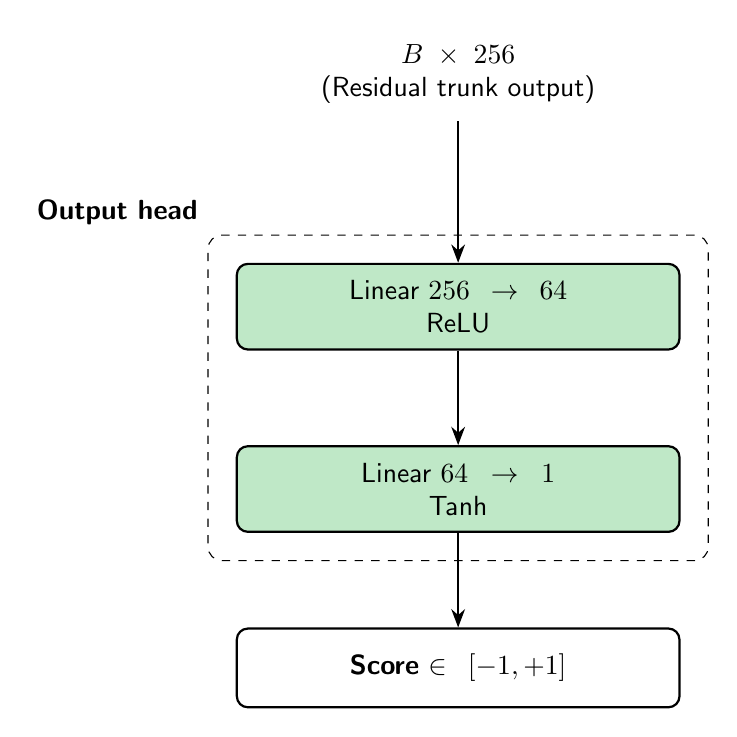
\begin{tikzpicture}[
    >=Stealth,
    thick,
    font=\sffamily,
    node distance=1.4cm and 1.6cm,
    block/.style={
        draw,
        rounded corners=4pt,
        align=center,
        minimum height=1.0cm,
        text width=5.2cm,
        inner sep=6pt
    },
    merge/.style={block, fill=none, draw=none},
    output_head/.style={block, fill=output_head},
    output/.style={block, fill=none},
    groupbox/.style={
        draw,
        rounded corners=5pt,
        dashed,
        inner sep=10pt,
        label={[font=\bfseries\sffamily]north west:#1}
    }
]

\node[merge] (H) {$B \times 256$\\(Residual trunk output)};
\node[output_head, below=1.8cm of H] (O1) {Linear $256\to64$\\ReLU};
\node[output_head, below=1.2cm of O1] (O2) {Linear $64\to1$\\Tanh};
\node[output, below=1.2cm of O2] (Score) {\textbf{Score $\in [-1,+1]$}};

\draw[->] (H) -- (O1);
\draw[->] (O1) -- (O2);
\draw[->] (O2) -- (Score);

\begin{scope}[on background layer]
    \node[groupbox=Output head, fit=(O1)(O2)] {};
\end{scope}

\end{tikzpicture}

\end{document}
